% 2013 湖南卷理科第 11 题：圆 O 中弦 AB 与 CD 交于 P（TikZ 矢量重绘）。
% 半径 sqrt(7)，P(0,sqrt3)，A(-2,sqrt3)，B(2,sqrt3)，D(1/2,3sqrt3/2)，C(-2,-sqrt3)。
% 此时 PA=PB=2，PD=1，PC=4，CD=5。
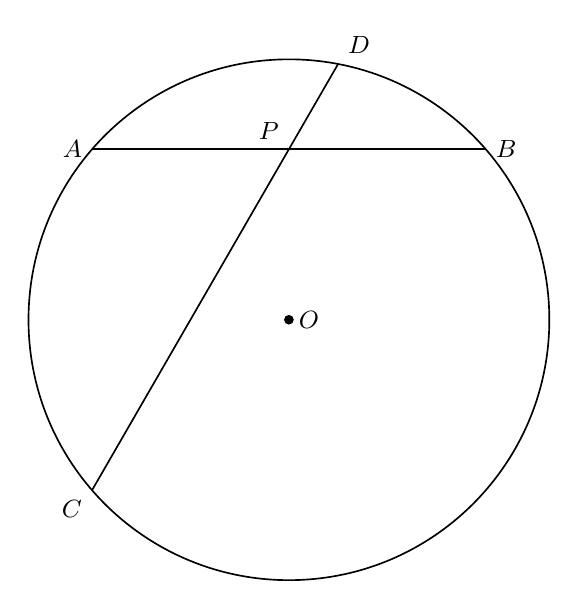
\begin{tikzpicture}[scale=1.25, font=\small, line width=0.6pt]
  \coordinate (O) at (0,0);
  \coordinate (P) at (0,1.7321);
  \coordinate (A) at (-2,1.7321);
  \coordinate (B) at (2,1.7321);
  \coordinate (D) at (0.5,2.5981);
  \coordinate (C) at (-2,-1.7321);

  \draw (O) circle ({sqrt(7)});
  \draw (A) -- (B);
  \draw (C) -- (D);

  \fill (O) circle (1.4pt);
  \node[right] at (O) {$O$};
  \node[above left] at (P) {$P$};
  \node[left] at (A) {$A$};
  \node[right] at (B) {$B$};
  \node[above right] at (D) {$D$};
  \node[below left] at (C) {$C$};
\end{tikzpicture}
